\section{Results and Analysis}
\label{sec:results}

\subsection{RQ1: Profile-Discordance is Prevalent and Structural}
\label{sec:results:rq1}

We characterise discordance in four slices, starting from the pooled transaction rate and drilling into the customer, band, and year dimensions in turn. At the transaction level (Figure~\ref{fig:rq1-dist}), of 228{,}241 scoreable Buys:
\begin{enumerate}
    \item 18.6\% violate the declared band by two or more steps.
    \item 81.4\% are coherent, of which 34.1\% strictly ($d = 0$).
    \item Mean discordance is 0.874 bands across all scoreable Buys, indicating that when mismatches occur they are usually a single band step.
\end{enumerate}

\begin{figure}[H]
    \centering
    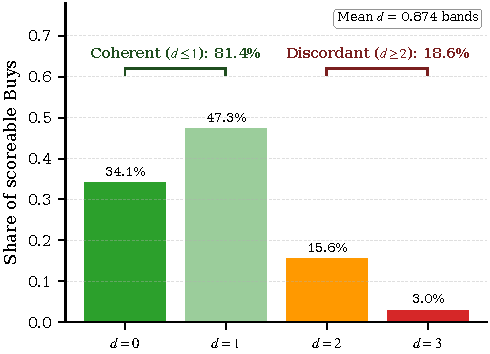
\includegraphics[width=\linewidth]{figures/rq1_discordance_distribution.pdf}
    \caption{Distribution of pairwise discordance $d$ over 228{,}241 scoreable Buys. Most mass sits at $d \leq 1$ (coherent), with non-negligible density at $d \geq 2$ (discordant).}
    \label{fig:rq1-dist}
\end{figure}

The pooled rate cannot tell us whether these violations are i.i.d.\ transaction-level slips spread thinly across the customer base or a structural trait concentrated in a subset. Slicing by customer settles the question. The per-customer discordant share (Figure~\ref{fig:rq1-self}) is sharply bimodal at 0\% and 100\% rather than clustering near the 19\% mean. More explicitly, 64.4\% of banded customers are fully coherent across every Buy and 17.2\% are fully discordant. An i.i.d.\ noise process cannot produce this shape, making discordance a persistent customer-level trait.

\begin{figure}[H]
    \centering
    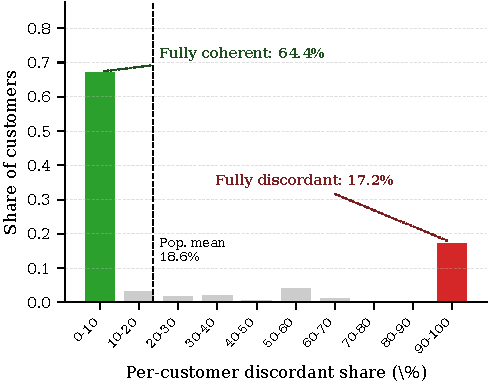
\includegraphics[width=\linewidth]{figures/rq1_self_discordance.pdf}
    \caption{Per-customer share of discordant Buys is sharply bimodal at 0\% and 100\%, ruling out i.i.d.\ transaction-level noise.}
    \label{fig:rq1-self}
\end{figure}

If the trait is customer-level, the next question is which customers carry it. Coherence per declared band is U-shaped (Figure~\ref{fig:rq1-per-band}): Conservative at 45.1\% (possibly reflecting a ``reach for yield'' tendency), Aggressive at 56.2\% (possibly reflecting a regression toward safer assets), with the two centre bands at $\sim$90\%. The two ordinal extremes carry most of the mismatch while the centre bands are nearly fully coherent, which corroborates the bimodality finding from the customer slice.

\begin{figure}[H]
    \centering
    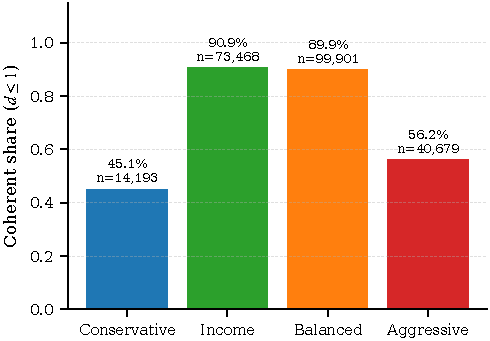
\includegraphics[width=\linewidth]{figures/rq1_per_band_coherence.pdf}
    \caption{Coherence share by declared band. The U-shape supports the bimodality result of Figure~\ref{fig:rq1-self}: discordance concentrates on the ordinal extremes.}
    \label{fig:rq1-per-band}
\end{figure}

A final slice rules out a regime-driven artefact. Mean discordance is flat across 2019 to 2022 (within 0.02 bands, see Figure~\ref{fig:rq1-yearly}), so the pattern is not the product of any single year's market conditions. The 2018 value (0.98) sits higher but covers a small slice. MiFID II came into force on 2018-01-03, the exact start of FAR-Trans, so we hypothesise the elevation as a transition effect. However this hypothesis is not tested and is potential future work.

\begin{figure}[H]
    \centering
    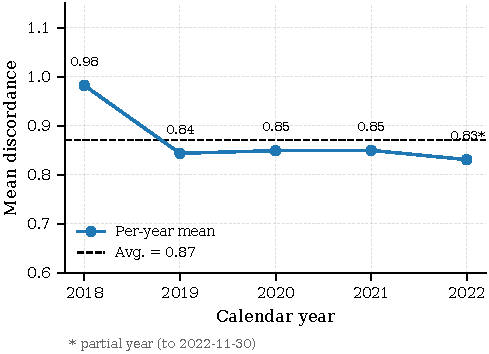
\includegraphics[width=\linewidth]{figures/rq1_yearly_discordance.pdf}
    \caption{Mean discordance by calendar year. The 2019 to 2022 cluster sits within 0.02 bands, with 2018 elevated (transition-effect hypothesis).}
    \label{fig:rq1-yearly}
\end{figure}

\subsection{RQ2: Coherent Buys Earn a Conditional Return Premium}
\label{sec:results:rq2}

The model from Section~\ref{sec:setup:stats} is fit on 208{,}029 priced Buys with cluster-robust SE on \texttt{customerID}. Table~\ref{tab:rq2-full} reports the full coefficient table.

\begin{table*}[!t]
\centering
\small
\begin{tabular}{lrrrr}
\toprule
Term & Estimate & Std.\ Error & 95\% CI & $p$ \\
\midrule
Intercept                                & $-0.0471$ & $0.0141$ & $[-0.0746,\; -0.0195]$ & $8.1 \times 10^{-4}$ \\
\texttt{is\_coherent}                    & $+0.0294$ & $0.0040$ & $[+0.0215,\; +0.0372]$ & $2.3 \times 10^{-13}$ \\
\texttt{asset\_volatility}               & $-0.1025$ & $0.0165$ & $[-0.1349,\; -0.0701]$ & $5.5 \times 10^{-10}$ \\
\texttt{C(customer\_type)[Legal Entity]} & $+0.0154$ & $0.0486$ & $[-0.0798,\; +0.1106]$ & $0.751$ \\
\texttt{C(customer\_type)[Mass]}         & $+0.0011$ & $0.0132$ & $[-0.0248,\; +0.0269]$ & $0.936$ \\
\texttt{C(customer\_type)[Premium]}      & $+0.0058$ & $0.0135$ & $[-0.0206,\; +0.0322]$ & $0.667$ \\
\texttt{C(customer\_type)[Professional]} & $+0.0247$ & $0.0169$ & $[-0.0084,\; +0.0578]$ & $0.143$ \\
\texttt{C(year)[2019]}                   & $+0.1759$ & $0.0129$ & $[+0.1507,\; +0.2012]$ & $1.4 \times 10^{-42}$ \\
\texttt{C(year)[2020]}                   & $+0.2107$ & $0.0061$ & $[+0.1986,\; +0.2227]$ & $6.2 \times 10^{-259}$ \\
\texttt{C(year)[2021]}                   & $+0.0754$ & $0.0053$ & $[+0.0651,\; +0.0858]$ & $4.1 \times 10^{-46}$ \\
\texttt{C(year)[2022]}                   & $-0.0195$ & $0.0045$ & $[-0.0283,\; -0.0107]$ & $1.4 \times 10^{-5}$ \\
\bottomrule
\end{tabular}
\caption{Full RQ2 OLS coefficient table on 208{,}029 priced Buys, cluster-robust SE on \texttt{customerID}. Reference cell: Inactive customer, 2018, $\texttt{asset\_volatility} = 0$, $\texttt{is\_coherent} = 0$.}
\label{tab:rq2-full}
\end{table*}

Coherent Buys earn $+2.94$ percentage points (pp) higher 6-month realised return than discordant ones, conditional on volatility, segment, and year. The positive sign with $p < 10^{-12}$ provides strong evidence against the prior that regulatory coherence imposes a return tax. The raw slice gap is $+3.31$ pp, so controls absorb only $\sim$0.4 pp ($\sim$11\% of the unconditional gap). This implies that coherence is not a volatility, segment, or year confound. However, it is important to note that unobserved confounders (financial literacy, advisor channel, account constraints) are not ruled out.

The volatility coefficient is $-10.3$ pp per unit, consistent with low-volatility outperformance over 2019 to 2022 and the 2022 rate shock that hit high-beta names. All four year dummies reject $H_0$: 2020 strongly positive (COVID rebound) and 2022 negative (Fed-hike bond drawdown). All four \texttt{customerType} dummies fail to reject $H_0$: segmentation contributes no detectable return signal, and together with RQ1's bimodality it does not capture the persistent customer-level discordance trait either.

\subsection{RQ3: Both Baselines Under-Serve at Least One Band}
\label{sec:results:rq3}

At primary-metric optima (Table~\ref{tab:rq3-aggregate}), LightGCN wins ranking quality (nDCG 0.330, Recall 0.495, PC@10 0.794) but loses ROI ($-0.5$\%/mo). Conversely, Random Forest wins ROI ($+1.4$\%/mo) but ranks near random on nDCG (0.019) and Recall (0.036). Both look fine on aggregate PC (LightGCN PC-lift $1.17\times$, Random Forest $1.06\times$), but the aggregate hides per-band failures.

\begin{table}[H]
\centering
\small
\begin{tabular}{lrrrr}
\toprule
Model & nDCG@10 & ROI@10 & Recall@10 & PC@10 \\
\midrule
LightGCN      & $0.330$ & $-0.005$ & $0.495$ & $0.794$ \\
RF            & $0.019$ & $+0.014$ & $0.036$ & $0.667$ \\
\bottomrule
\end{tabular}
\caption{RQ3 aggregate metrics at primary-metric optima, averaged over 69 splits. ROI@10 is per-month.}
\label{tab:rq3-aggregate}
\end{table}

Table~\ref{tab:per-band-rq3} decomposes PC@10 by declared band. Per-band lift moves $0.75 \to 1.13 \to 1.17 \to 1.35$ for LightGCN and $0.52 \to 0.70 \to 1.03 \to 1.88$ for Random Forest across Conservative~$\to$~Income~$\to$~Balanced~$\to$~Aggressive. For both, lift rises monotonically with the declared band: recommended assets skew higher-risk. LightGCN's range is flatter, which we attribute to its per-user embeddings shifting each customer's top-$k$ partly toward their tolerance window. Recall that Random Forest carries no customer signal.

\begin{table}[H]
\centering
\footnotesize
\setlength{\tabcolsep}{4pt}
\begin{tabular}{llrrrr}
\toprule
Band & Model & N & $\pi(b)$ & PC@10 & PC-lift@10 \\
\midrule
Conservative & RF       & 5{,}348  & $0.65$ & $0.34$ & $0.52$ \\
Conservative & LightGCN & 5{,}348  & $0.65$ & $0.48$ & $0.75$ \\
Income       & RF       & 45{,}142 & $0.78$ & $0.54$ & $0.70$ \\
Income       & LightGCN & 45{,}142 & $0.78$ & $0.88$ & $1.13$ \\
Balanced     & RF       & 61{,}181 & $0.76$ & $0.79$ & $1.03$ \\
Balanced     & LightGCN & 61{,}181 & $0.76$ & $0.89$ & $1.17$ \\
Aggressive   & RF       & 25{,}367 & $0.35$ & $0.66$ & $1.88$ \\
Aggressive   & LightGCN & 25{,}367 & $0.35$ & $0.47$ & $1.35$ \\
\bottomrule
\end{tabular}
\caption{Per-band PC@10 and PC-lift@10 versus the band-conditional random baseline $\pi(b)$ for the two FAR-Trans baselines at their primary-metric optima, aggregated over 69 splits. PC-lift@10 = PC@10 / $\pi(b)$.}
\label{tab:per-band-rq3}
\end{table}

By customer footprint, LightGCN under-serves the 19.7\% Conservative segment while Random Forest under-serves 60.9\% (Conservative and Income combined). Aggressive's high lift is partly mechanical: $\pi(\text{Aggressive}) = 0.35$ is the lowest band, so any model skewing higher-volatility clears that bar easily. Neither baseline has band labels or a band-aware loss, so per-band coherence is a passive byproduct of training rather than a controlled output.

\subsection{RQ4: Stratification + PC-Loss Closes the Per-Band Deficit}
\label{sec:results:rq4}

PC-LightGCN (Section~\ref{sec:method:pclgcn}) addresses the RQ3 gap by routing each customer to a band-stratified sub-model and adding a coherence margin to the BPR objective. Table~\ref{tab:rq4-aggregate} reports aggregate metrics for the baseline LightGCN, the $\lambda = 0$ ablation (stratification only), and the $\lambda = 1$ treatment (stratification plus the coherence margin) over 69 splits. The treatment lifts PC@10 from $0.794$ to $0.918$, a $+12.4$ pp gain, and PC-lift from $1.17\times$ to $1.40\times$. Figure~\ref{fig:rq4-winrate} confirms this is not a split-averaging artefact: the treatment achieves a 100\% win rate on PC@10 across all 69 splits.

\begin{figure}[H]
    \centering
    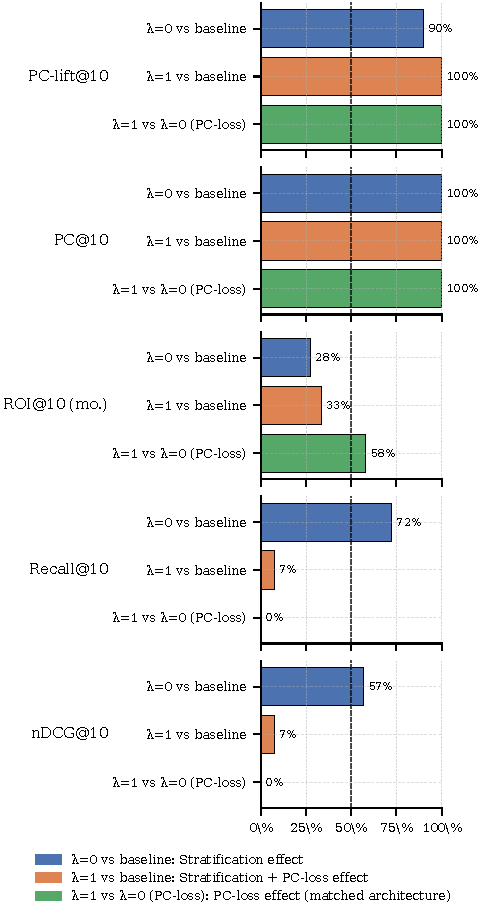
\includegraphics[width=\linewidth]{figures/rq4_paired_win_rates.pdf}
    \caption{Per-split win rates of the $\lambda = 0$ and $\lambda = 1$ trials against the global LightGCN baseline.}
    \label{fig:rq4-winrate}
\end{figure}

\begin{table*}[!t]
\centering
\small
\begin{tabular}{lrrrrr}
\toprule
Trial & nDCG@10 & ROI@10 & Recall@10 & PC@10 & PC-lift@10 \\
\midrule
Baseline LightGCN      & $0.330$ & $-0.005$ & $0.495$ & $0.794$ & $1.17\times$ \\
$\lambda = 0$ & $0.332$ & $-0.007$ & $0.501$ & $0.821$ & $1.19\times$ \\
$\lambda = 1$ & $0.309$ & $-0.007$ & $0.467$ & $0.918$ & $1.40\times$ \\
\bottomrule
\end{tabular}
\caption{RQ4 aggregate metrics, averaged over 69 splits. ROI@10 is per-month. PC-lift@10 is PC@10 divided by the band-conditional random baseline $\pi(b)$, expressed as a multiple.}
\label{tab:rq4-aggregate}
\end{table*}

Because the treatment bundles two architectural changes, the $\lambda = 0$ ablation lets us attribute the $+12.4$ pp PC@10 gain to each piece. The paired per-split deltas in Figure~\ref{fig:rq4-deltas} read as follows. Stratification alone supplies $+2.7$ pp of PC@10, about a quarter of the full gain. The accompanying nDCG ($+0.002$, 57\% win rate), Recall ($+0.006$, 72\% win rate), and ROI ($-0.002$ pp/mo, 28\% win rate) movements sit close enough to zero that none of them registers as a real effect. Adding the PC-loss on top buys the remaining $+9.7$ pp of PC@10, three quarters of the total gain, winning it on every split. The cost is roughly $-2$ pp of nDCG and $-3$ pp of Recall, also lost on every split. Stratification is therefore the cheap component of the intervention, and the PC-loss carries the bulk of the gain at a measurable but bounded ranking cost.

\begin{figure}[H]
    \centering
    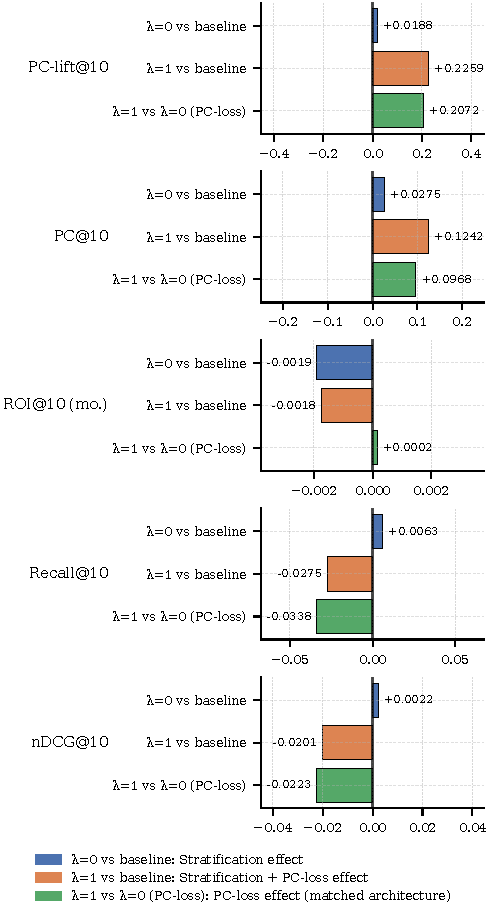
\includegraphics[width=\linewidth]{figures/rq4_paired_deltas.pdf}
    \caption{Paired per-split deltas of $\lambda = 1$ vs baseline LightGCN. PC@10 is positive on every one of 69 splits.}
    \label{fig:rq4-deltas}
\end{figure}

Aggregate ROI is essentially flat across all three trials. The paired ROI deltas in Figure~\ref{fig:rq4-deltas} are $-0.002$ pp/mo for both the stratification ablation and the full treatment against baseline, and a near-zero $+0.0001$ pp/mo for the PC-loss step on its own. The small ROI cost therefore lives in the stratification step rather than the coherence margin, and is too small to read off the aggregate row of Table~\ref{tab:rq4-aggregate}.

Together with RQ2's coherence premium, this null aggregate-ROI effect indicates that the recommender can be made meaningfully more profile-coherent without giving up the return story. This reframes coherence as an architectural choice rather than a post-hoc tradeoff.
